\documentclass[10 pt,usenames,dvipsnames, oneside]{article}
\usepackage{../../modelo-fracoes}
\graphicspath{{../../../Figuras/licao01/}}



\begin{document}

\begin{center}
  \begin{minipage}[l]{3cm}

\includegraphics[width=2cm]{../../../Figuras/logo}       
\end{minipage}\hfill
\begin{minipage}[r]{.8\textwidth}
 {\Large \scshape Atividade: Repartindo três pizzas na turma}  
\end{minipage}
\end{center}
\vspace{.2cm}

\ifdefined\prof
\begin{goals}
\begin{enumerate}

\item       Perceber que uma unidade (no caso, uma pizza) pode ser subdividida em um mesmo número de partes sem que cada divisão represente uma equipartição.
\item       Distinguir uma equipartição dentre partições diversas.
\item       Diferenciar       ``a divisão da unidade em quatro partes quaisquer'' da       ``divisão da unidade em quatro partes iguais''.
\item       Compreender as expressões ``um quarto de'' e ``quarta parte de'' como forma de identificar uma das partes da equipartição em 4 partes.
\end{enumerate}
\tcblower

  \begin{itemize} %s
    \item No final deste volume estão disponíveis materiais para reprodução.
    \item Recomenda-se que a atividade seja desenvolvida em grupos de 3 a 5 alunos.
    \item As diversas soluções apresentadas pelos diferentes grupos devem ser discutidas com a turma inteira.
    \item É importante que a discussão conduza os alunos ao entendimento de que apenas as partes da equipartição podem ser chamadas de ``quartos'' da pizza, as demais são simplesmente fatias ou pedaços, por exemplo.
    \item Os alunos devem reconhecer que, apesar de todas as pizzas estarem repartidas em quatro fatias, apenas uma das repartições propostas sugere a equipartição, respondendo assim a último item desta atividade.
    \item       Essa atividade pode ser adaptada visando à inclusão de alunos com deficiência visual. Para isso, sugere-se confeccionar os modelos das três pizzas repartidas, que estão disponíveis para reprodução no final do livro, em três materiais diferentes. Por exemplo, papel comum e papéis com texturas diferentes, tecido ou material emborrachado.
\end{itemize} %s

\end{goals}

\bigskip
\begin{center}
{\large \scshape Atividade}
\end{center}
\fi

Três pizzas inteiras, de mesmo tamanho, foram repartidas entre as crianças de uma turma. Para isso, a turma foi dividida em três grupos com quatro crianças cada. Veja como cada grupo repartiu a sua pizza.

\begin{center}
    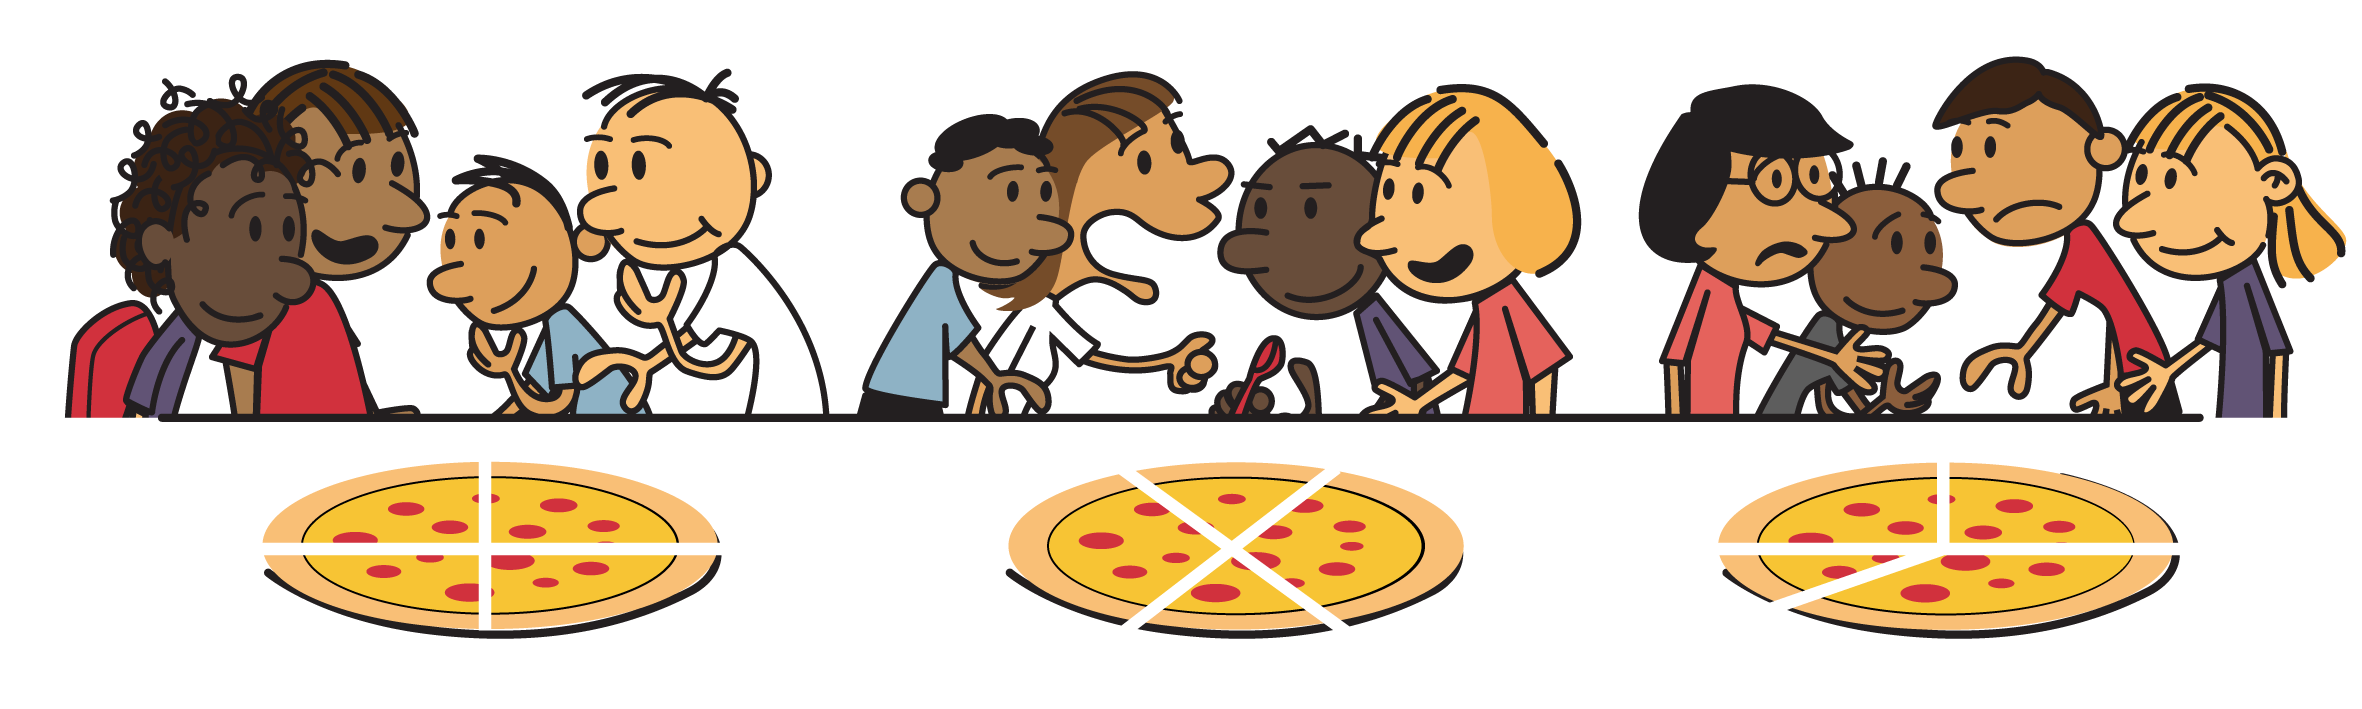
\includegraphics[width=400pt, keepaspectratio]{ativ2_fig01.png}

    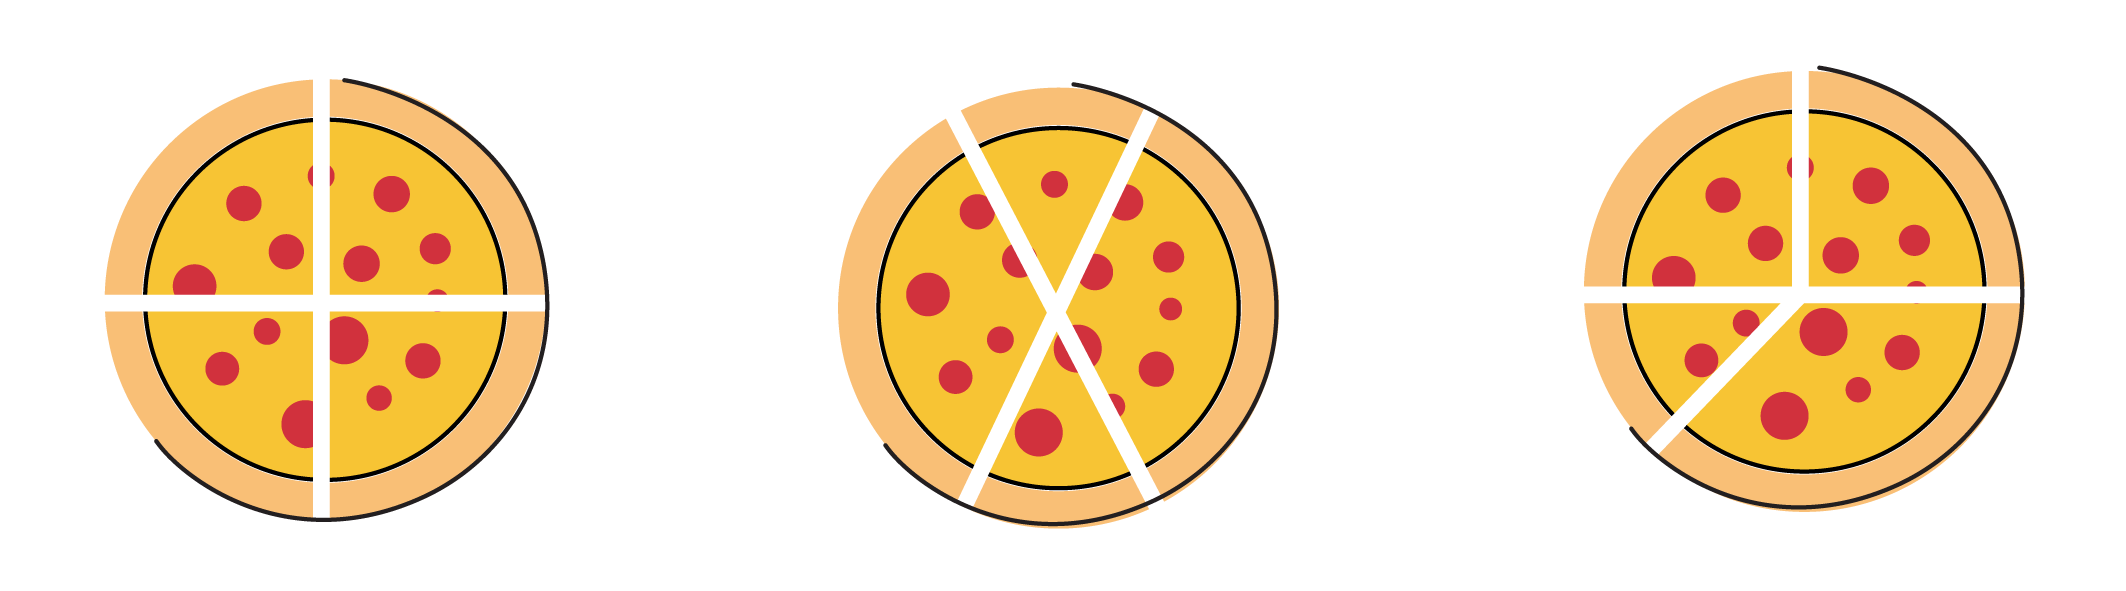
\includegraphics[width=300pt, keepaspectratio]{ativ2_fig02.png}
\end{center}

\begin{enumerate}[label=\alph*)] %d
  \item Cada um dos três grupos repartiu a sua pizza na mesma \textbf{quantidade de fatias} que os outros grupos?
  \item Dessa maneira, todas as crianças da turma receberam a mesma \textbf{quantidade de pizza}?
  \item É verdade que em algum dos grupos, as 4 crianças receberam a mesma quantidade de pizza? Se sim, em qual? Considerando a pizza inteira, como você nomearia cada uma das fatias de pizza desse grupo?
\end{enumerate} %d

\ifdefined\prof

\begin{solucao}

\begin{enumerate}[label=\alph*),wide,labelindent=0pt] %d
    \item       Sim. Cada grupo repartiu sua pizza em quatro fatias.
    \item       Não, pois algumas fatias têm quantidades de pizza diferentes das outras.
    \item       Apenas no grupo 1 as 4 crianças receberam a mesma quantidade de pizza. Cada fatia da pizza do grupo 1 é {\it um quarto} da pizza ou {\it a quarta parte} da pizza.
\end{enumerate} %d

\end{solucao}
\fi

\end{document}